\documentclass[10pt,twoside]{article}
\usepackage[T1]{fontenc}
\usepackage[utf8]{inputenc}
\usepackage{helvet}
\renewcommand{\familydefault}{\sfdefault}
\usepackage{geometry}
\geometry{paperwidth=6.93in,paperheight=9.11in,inner=0.56in,outer=0.46in,top=0.66in,bottom=0.66in,headheight=14pt}
\usepackage{array}
\usepackage{booktabs}
\usepackage{longtable}
\usepackage{tabularx}
\usepackage{xcolor}
\usepackage{fancyhdr}
\usepackage{titlesec}
\usepackage{enumitem}
\usepackage{needspace}
\usepackage{tikz}
\usetikzlibrary{arrows.meta}
\usepackage{hyperref}
\hypersetup{colorlinks=true,linkcolor=black,urlcolor=black,pdfauthor={ISA tooling},pdftitle={Bedrock C ABI}}
\makeatletter
\renewcommand{\@pnumwidth}{2.2em}
\renewcommand{\@tocrmarg}{3.0em}
\makeatother
\definecolor{RuleGray}{gray}{0.18}
\setlength{\parindent}{0pt}
\setlength{\parskip}{4pt}
\setlength{\tabcolsep}{3pt}
\sloppy
\emergencystretch=2em
\clubpenalty=10000
\widowpenalty=10000
\displaywidowpenalty=10000
\brokenpenalty=10000
\raggedbottom
\setlist[itemize]{leftmargin=1.0em,itemsep=1pt,topsep=2pt}
\renewcommand{\arraystretch}{1.14}
\pagestyle{fancy}
\fancyhf{}
\fancyhead[LE]{\small Bedrock}
\fancyhead[RO]{\small REFERENCE ABI}
\fancyfoot[LE,RO]{\small\thepage}
\fancyfoot[LO,RE]{\small Bedrock ABI}
\titleformat{\section}{\Large\bfseries}{\thesection}{0.6em}{}
\titleformat{\subsection}{\large\bfseries}{\thesubsection}{0.55em}{}
\titlespacing*{\section}{0pt}{1.3em}{0.45em}
\titlespacing*{\subsection}{0pt}{0.9em}{0.25em}
\newcommand{\manualtablecaption}[1]{\par\Needspace{1.25in}\refstepcounter{table}\addcontentsline{lot}{table}{\protect\numberline{\thetable}#1}{\small\bfseries Table \thetable. #1\par\vspace{2pt}}}
\newcommand{\manualfield}[2]{\Needspace{0.45in}\noindent\begin{tabularx}{\linewidth}{@{}p{1.25in}X@{}}\textbf{#1} & #2\end{tabularx}\par}
\begin{document}


\begin{titlepage}
\centering
\vspace*{0.75in}
{\Large BEDROCK ARCHITECTURE\par}
\vspace{0.25in}
{\Huge\bfseries Bedrock C ABI\par}
\vspace{0.30in}
{\large C Language Binding\par}
\vspace{0.20in}
{\large Version 0.1\par}
\vfill
\end{titlepage}
\pagenumbering{roman}
\tableofcontents
\clearpage
\listoftables
\clearpage
\pagenumbering{arabic}


\clearpage
\section{Scope and Profiles}
The Bedrock C ABI defines the C data model, register convention, function call contract, aggregate passing rules, variadic call rules, return-value assignment, and compiler-runtime obligations for C-family toolchains. It builds on the Bedrock language-neutral ELF ABI for object files, relocation, loading, dynamic linking, TLS, and code models.
\subsection{ABI Hierarchy}
\Needspace{2.7in}
\begin{center}
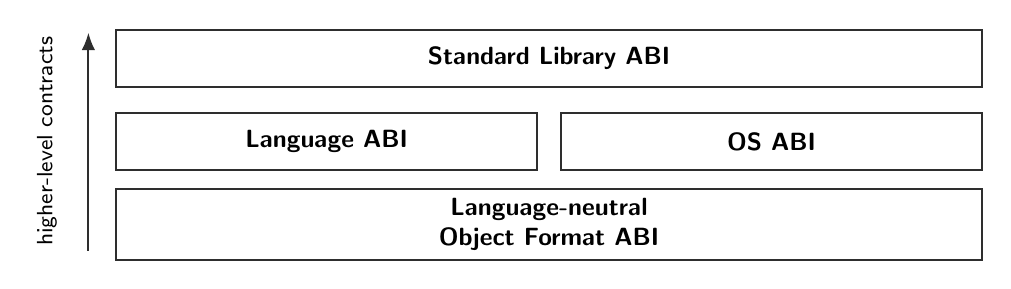
\begin{tikzpicture}[
  abiLayerBox/.style={draw=RuleGray, fill=white, line width=0.75pt, minimum height=0.72cm, align=center, font=\small\bfseries},
  currentAbiLayerBox/.style={abiLayerBox, fill=black!12, line width=1.15pt},
  abiAxis/.style={-{Latex[length=2.2mm,width=1.7mm]}, draw=RuleGray, line width=0.65pt}
]
\node[abiLayerBox, minimum width=11.0cm, text width=10.4cm] (standard) at (0,2.10) {Standard Library ABI};
\node[abiLayerBox, minimum width=5.35cm, text width=4.8cm] (language) at (-2.825,1.05) {Language ABI};
\node[abiLayerBox, minimum width=5.35cm, text width=4.8cm] (os) at (2.825,1.05) {OS ABI};
\node[abiLayerBox, minimum width=11.0cm, text width=10.4cm] (object) at (0,0.00) {Language-neutral\\Object Format ABI};
\draw[abiAxis] (-5.85,-0.34) -- (-5.85,2.43);
\node[font=\footnotesize, rotate=90, anchor=south] at (-6.13,1.05) {higher-level contracts};
\end{tikzpicture}
\end{center}
\noindent\textbf{Current document.} This document specifies one language ABI layer: the Bedrock C language binding. It relies on the language-neutral ELF ABI for object files, relocation, loading, dynamic linking, TLS, and code models, while leaving process-entry policy to an OS ABI.
\subsection{ABI Profiles}
\manualtablecaption{Reference ABI Profiles}
\begingroup\footnotesize
\setlength{\tabcolsep}{2pt}
\begin{longtable}{@{}p{1.35in}p{4.15in}@{}}
\toprule
\textbf{Profile} & \textbf{Meaning}\\
\midrule
\endhead
\texttt{bedrock-c} & C-family language binding layered on the Bedrock language-neutral ELF ABI.\\
\bottomrule
\end{longtable}
\endgroup

\clearpage
\section{Terminology}
These terms are specific to the C binding. ELF and address-space terms keep the meanings defined by the language-neutral ABI and the architecture manual.
\begin{description}[style=nextline,leftmargin=1.45in,labelwidth=1.35in,itemsep=3pt,topsep=3pt]
\item[object pointer] A 64-bit pre-segment address value that designates an object or one-past an object according to the C abstract machine.
\item[function pointer] A 64-bit pre-segment code address naming a near-call entry point. It is not a CS:PC pair, far descriptor, or runtime-private veneer descriptor.
\item[caller-saved register] A register whose value may be overwritten by a call unless the caller saves it before the call.
\item[callee-saved register] A register whose incoming value must be preserved by the called function if the function uses it.
\item[sret buffer] Caller-allocated storage used to receive a return value that is too large or unsuitable for the normal return registers.
\item[addressable by-value argument] A by-value aggregate argument that is passed through caller-owned stack storage because the callee may need an address for the object.
\end{description}







\clearpage
\section{Data Model}
\manualfield{Model:}{LP64}
\manualfield{Byte Order:}{little endian}
\manualfield{Instruction Word:}{16 bits}
\manualfield{Stack Alignment:}{16 bytes}
\manualfield{Aggregate Maximum Alignment:}{16 bytes}
\subsection{Scalar Types}
\manualtablecaption{Reference C Data Model}
\begingroup\footnotesize
\setlength{\tabcolsep}{2pt}
\begin{longtable}{@{}p{2.1in}p{1.0in}p{1.0in}@{}}
\toprule
\textbf{Type} & \textbf{Bits} & \textbf{Align}\\
\midrule
\endhead
\texttt{\_\allowbreak{}Bool} & 8 & 1\\
\texttt{char} & 8 & 1\\
\texttt{signed char} & 8 & 1\\
\texttt{unsigned char} & 8 & 1\\
\texttt{short} & 16 & 2\\
\texttt{int} & 32 & 4\\
\texttt{long} & 64 & 8\\
\texttt{long long} & 64 & 8\\
\texttt{\_\allowbreak{}\_\allowbreak{}int128} & 128 & 16\\
\texttt{unsigned \_\allowbreak{}\_\allowbreak{}int128} & 128 & 16\\
\texttt{pointer} & 64 & 8\\
\texttt{size\_\allowbreak{}t} & 64 & 8\\
\texttt{ptrdiff\_\allowbreak{}t} & 64 & 8\\
\texttt{wchar\_\allowbreak{}t} & 32 & 4\\
\texttt{char16\_\allowbreak{}t} & 16 & 2\\
\texttt{char32\_\allowbreak{}t} & 32 & 4\\
\texttt{float} & 32 & 4\\
\texttt{double} & 64 & 8\\
\texttt{long double} & 64 & 8\\
\bottomrule
\end{longtable}
\endgroup
\subsection{Layout Rules}
\begin{itemize}
\item Integer and pointer objects are stored little-endian.
\item Plain char is signed. signed char, unsigned char, and plain char remain distinct C types.
\item The default enum representation is the 32-bit int representation with 4-byte alignment.
\item  Bool stores canonical values as 0 or 1 in bit 0; upper bits are ignored by consumers.
\item   int128 and unsigned   int128 objects are stored little-endian; the low 64 bits live at the lower address.
\item long double uses the same 8-byte IEEE-754 binary64 storage format as double.
\item Pointer values are pre-segment virtual address values. Memory accesses apply segment pre-translation when the pointer is used as part of an effective address.
\item C function pointers are ordinary 64-bit pre-segment code addresses naming near-call entry points. They are not CS:PC pairs or far-call descriptors.
\item Object pointers and function pointers have the same size and alignment but remain distinct C pointer categories.
\item Multiword immediate data and data directives store the least significant 16-bit word first.
\item Struct fields are laid out in declaration order with natural alignment up to the aggregate maximum.
\item Unions have the size and alignment of their most strictly aligned member, rounded up to that alignment.
\item Arrays store elements contiguously with each element using the ABI size of its type.
\item Aggregate object size is rounded up to the aggregate object's alignment.
\item Boolean objects store the truth value in bit 0; upper bits are ignored by consumers.
\end{itemize}

\clearpage
\section{Register Convention}
\manualtablecaption{Register Preservation and Assignment}
\begingroup\footnotesize
\setlength{\tabcolsep}{2pt}
\begin{longtable}{@{}p{1.35in}p{1.55in}p{2.6in}@{}}
\toprule
\textbf{Group} & \textbf{Rule} & \textbf{Registers / Meaning}\\
\midrule
\endhead
integer registers & caller saved & D0, D1, D2, D3, D4, D5\\
integer registers & callee saved & D6, D7\\
integer registers & c scalar return & D0\\
integer registers & c 128 bit scalar return & D1:D0\\
integer registers & integer arguments & D0, D1, D2, D3, D4, D5\\
address registers & caller saved & A0, A1, A2, A3, A4, A5\\
address registers & callee saved & A6, A7\\
address registers & pointer arguments & A0, A1, A2, A3, A4, A5\\
address registers & c pointer return & A0\\
address registers & conditional sret buffer argument & A5\\
address registers & sret result return & A0\\
floating point registers & caller saved & F0, F1, F2, F3, F4, F5, F6, F7\\
floating point registers & callee saved & \begin{tabular}[t]{@{}l@{}}F8\\F9\\F10\\F11\\F12\\F13\\F14\\F15\end{tabular}\\
floating point registers & callee save mechanism & instruction pair: FPUSHM/FPOPM
bitmap rule: bits 0..15 name F0-F15; C ABI prologues and epilogues normally set only
  bits for clobbered F8-F15\\
floating point registers & floating point arguments & F0, F1, F2, F3, F4, F5, F6, F7\\
floating point registers & c floating point return & F0\\
stack register & name & SP\\
stack register & role & architectural stack pointer\\
stack register & preserved by callee & true\\
stack register & ordinary c use & stack pointer only; not available as a general C temporary\\
program counter & name & PC\\
program counter & role & architectural instruction pointer\\
program counter & ordinary c use & control-flow target only; not available as a general C temporary\\
flags & caller saved & FLAGS\\
flags & callee obligation & callees may clobber condition codes\\
status registers & STATUS & not part of the C abstract machine; ordinary C code may access it only through target-specific intrinsics or runtime code\\
status registers & FSTATUS & not part of the C abstract machine; floating-point environment support is a higher-level runtime contract\\
status registers & FFLAGS & not part of the C abstract machine; floating-point exception flag handling is a higher-level runtime contract\\
\bottomrule
\end{longtable}
\endgroup
\subsection{Data Register Banking}
The C ABI is DBANK-neutral. C function calls use bank zero as the ABI-visible D-register file; nonzero data-register banks are optional target resources for compiler-generated temporaries and specialized runtime code.
\manualtablecaption{C ABI Data Register Banking Rules}
\begingroup\footnotesize
\setlength{\tabcolsep}{2pt}
\begin{longtable}{@{}p{2.0in}p{3.5in}@{}}
\toprule
\textbf{Rule} & \textbf{Value}\\
\midrule
\endhead
public boundary & DBANK must be 0 on C function entry and return\\
call boundary & A caller must issue an ordinary C call with DBANK = 0; a callee must return with DBANK = 0\\
source language visibility & DBANK is not visible to the C abstract machine\\
bank zero & D0-D7 in bank 0 are the ABI-visible integer registers listed below\\
nonzero banks & caller-managed volatile scratch state when enabled by the target object attributes\\
preservation & no nonzero bank is callee-saved by the C ABI\\
live across call & C code must not keep a live value only in a nonzero DBANK across an ordinary C call\\
target feature gate & use of DBANK beyond zero requires the language-neutral ELF DBANK object attribute\\
\bottomrule
\end{longtable}
\endgroup
\noindent\textbf{Recommended compiler policy.}
\begin{itemize}
\item Do not use DBANK in the baseline C code-generation mode.
\item Enable DBANK use only under an explicit target feature or optimization option.
\item Prefer nonzero banks for leaf hot regions, spill-heavy loops, and REP or REPG lowering.
\item Restore DBANK to zero before calls, returns, tail calls, unwinding edges, and externally visible labels.
\end{itemize}

\clearpage
\section{Calling Convention}
\subsection{Stack and Calls}
The stack grows downward. An architectural \texttt{CALL} pushes an
8-byte return address at \texttt{[SP]}, and
callers align \texttt{SP} before the call so callee entry observes
16-byte alignment. The ABI reserves no red zone and no
mandatory outgoing argument home area. A callee that needs stricter local
alignment realigns its own frame and restores the incoming \texttt{SP} before
return.

\subsection{Argument Assignment}
Arguments are assigned in source order. Scalar integer values use the D-register
class, pointer and address values use the A-register class, and floating-point
values use the F-register class. Arguments that exhaust their register class are
placed in 16-byte stack slots.

\manualtablecaption{C Argument Register Classes}
\begingroup\footnotesize
\setlength{\tabcolsep}{2pt}
\begin{longtable}{@{}p{1.45in}p{4.05in}@{}}
\toprule
\textbf{Class} & \textbf{Registers}\\
\midrule
\endhead
Integer scalar & \texttt{D0}, \texttt{D1}, \texttt{D2}, \texttt{D3}, \texttt{D4}, \texttt{D5}\\
Pointer/address & \texttt{A0}, \texttt{A1}, \texttt{A2}, \texttt{A3}, \texttt{A4}, \texttt{A5}\\
Floating-point & \texttt{F0}, \texttt{F1}, \texttt{F2}, \texttt{F3}, \texttt{F4}, \texttt{F5}, \texttt{F6}, \texttt{F7}\\
\bottomrule
\end{longtable}
\endgroup

\manualtablecaption{C Stack Argument Rules}
\begingroup\footnotesize
\setlength{\tabcolsep}{2pt}
\begin{longtable}{@{}p{1.85in}p{3.65in}@{}}
\toprule
\textbf{Rule} & \textbf{Value}\\
\midrule
\endhead
Stack order & right to left\\
Slot size & 16 bytes\\
Slot alignment & 16 bytes\\
Narrow signed integer & sign-extend to 64 bits\\
Narrow unsigned integer and \texttt{\_Bool} & zero-extend to 64 bits\\
\texttt{\_\_int128} register pair & \texttt{D1:D0}, with low bits in \texttt{D0} and high bits in \texttt{D1}\\
\texttt{\_\_int128} stack alignment & 16 bytes\\
Stack value placement & low address bytes\\
\bottomrule
\end{longtable}
\endgroup

\subsection{C Return Values}
\manualtablecaption{C Return Register Assignment}
\begingroup\footnotesize
\setlength{\tabcolsep}{2pt}
\begin{longtable}{@{}p{2.15in}p{3.35in}@{}}
\toprule
\textbf{Result Class} & \textbf{Register Rule}\\
\midrule
\endhead
Integer scalar & \texttt{D0}\\
Pointer/address scalar & \texttt{A0}\\
Floating-point scalar & \texttt{F0}\\
\texttt{long double} scalar & \texttt{F0}\\
\texttt{\_\_int128} scalar & \texttt{D1:D0}\\
Small aggregate & \texttt{D1:D0}\\
Large aggregate & sret pointer in \texttt{A5}, result pointer returned in \texttt{A0}\\
\bottomrule
\end{longtable}
\endgroup

\subsection{Aggregate Passing}
By-value aggregate arguments are addressable call copies. The caller creates the
copy, passes its address, and keeps the copy valid until the call returns. Mixed
integer/floating-point aggregates, packed aggregates, bitfield-containing
aggregates, and under-aligned aggregates use the same addressable-copy argument
rule.

\manualtablecaption{Aggregate Argument and Return Rules}
\begingroup\footnotesize
\setlength{\tabcolsep}{2pt}
\begin{longtable}{@{}p{2.2in}p{3.3in}@{}}
\toprule
\textbf{Rule} & \textbf{Value}\\
\midrule
\endhead
By-value argument copy alignment & 16 bytes\\
Copy address registers & \texttt{A0}, \texttt{A1}, \texttt{A2}, \texttt{A3}, \texttt{A4}, \texttt{A5}\\
Aggregate register arguments & none\\
Small aggregate return & 16 bytes or smaller in \texttt{D1:D0}\\
Small aggregate byte layout & low address bytes D0 then D1\\
Large aggregate return buffer alignment & 16 bytes\\
sret hidden pointer register & \texttt{A5}\\
sret result return register & \texttt{A0}\\
\bottomrule
\end{longtable}
\endgroup

\subsection{Variadic Calls}
Fixed named arguments use the normal assignment rules. Unnamed variadic
arguments and old-style unprototyped call arguments are materialized in uniform
stack slots, so \texttt{va\_list} traversal does not depend on the fixed
argument register assignment.

\manualtablecaption{Variadic Argument Rules}
\begingroup\footnotesize
\setlength{\tabcolsep}{2pt}
\begin{longtable}{@{}p{2.0in}p{3.5in}@{}}
\toprule
\textbf{Rule} & \textbf{Value}\\
\midrule
\endhead
Variable arguments & stack only\\
Register save area & none\\
Variadic slot size & 16 bytes\\
Variadic slot alignment & 16 bytes\\
\texttt{long double} variable argument & 8-byte binary64 value in one 16-byte slot\\
Aggregate variable argument & copy address in slot\\
\texttt{va\_arg} alignment & 16 bytes\\
\texttt{va\_list} & next variadic stack slot pointer\\
\bottomrule
\end{longtable}
\endgroup














\clearpage
\section{Freestanding C Binding}
Freestanding C uses the Bedrock C data and call ABI together with the
language-neutral ELF ABI. It is sufficient for compiler output, static objects,
and runtime-provided helper calls, but it does not define process startup or a
hosted C library environment.

\subsection{Execution Boundary}
The ELF entry field remains an object-loading field. The initial stack,
\texttt{\_start} contract, argument vectors, environment vectors, auxiliary
vectors, and process-entry state are OS ABI responsibilities. Zero-fill for BSS
storage is provided by ELF program loading for the file-size to memory-size gap
in loadable segments.

\subsection{Compiler Runtime Helpers}
The baseline backend may expand simple \texttt{\_\_int128} operations into
64-bit instruction sequences. Multiplication, division, remainder, and
integer/floating-point conversions may instead lower to compiler-runtime helper
calls. The ABI fixes the helper call convention, not a hosted runtime library
surface: helper calls use the normal Bedrock C ABI, and \texttt{\_\_int128}
helper returns use \texttt{D1:D0}.

\manualtablecaption{\texttt{\_\_int128} Runtime Helper Names}
\begingroup\footnotesize
\setlength{\tabcolsep}{2pt}
\begin{longtable}{@{}p{2.25in}p{3.25in}@{}}
\toprule
\textbf{Operation} & \textbf{Helper}\\
\midrule
\endhead
Multiply & \texttt{\_\allowbreak{}\_\allowbreak{}multi3}\\
Signed divide & \texttt{\_\allowbreak{}\_\allowbreak{}divti3}\\
Unsigned divide & \texttt{\_\allowbreak{}\_\allowbreak{}udivti3}\\
Signed remainder & \texttt{\_\allowbreak{}\_\allowbreak{}modti3}\\
Unsigned remainder & \texttt{\_\allowbreak{}\_\allowbreak{}umodti3}\\
Shift left & \texttt{\_\allowbreak{}\_\allowbreak{}ashlti3}\\
Arithmetic shift right & \texttt{\_\allowbreak{}\_\allowbreak{}ashrti3}\\
Logical shift right & \texttt{\_\allowbreak{}\_\allowbreak{}lshrti3}\\
\bottomrule
\end{longtable}
\endgroup

Floating-point helper calls may be used when the selected target lacks a
hardware operation. Those calls also use the normal Bedrock C ABI.

\subsection{TLS and OS ABI Boundary}
TLS requires an OS ABI, loader profile, or runtime that initializes the
language-neutral TLS model. An unknown freestanding OS profile may leave TLS
unsupported. TLSDESC and TLS relocation semantics are owned by the
language-neutral ELF ABI and resolved by the linker, loader, or OS ABI.

\subsection{C Linkage}
C function pointers are 64-bit pre-segment near-call code addresses. Code and
data pointers have the same size and alignment but remain distinct C pointer
categories. Common symbols and externally visible objects are aligned to at
least the ABI alignment of their declared type, subject to the aggregate maximum
unless stricter alignment is explicitly requested. Direct C calls use
\texttt{R\_\allowbreak{}BEDROCK\_\allowbreak{}CALL\_\allowbreak{}TARGET}; PLT-bound external calls use the PLT relocation
selected by the active code model.

Instruction relaxation is assembler and linker policy under the active code
model. Hosted C library entry points, process environment, filesystem behavior,
and syscall bindings are outside the freestanding C ABI.


\clearpage
\section{C Memory Model}
The C ABI defines the memory guarantees that C-family toolchains may assume
when lowering normal memory accesses, C atomic operations, volatile accesses,
and compiler-runtime helper calls. It does not define device ordering policy or
process-wide memory mapping policy.

\subsection{Normal Memory}
Naturally aligned 1, 2, 4, and 8 byte normal-memory loads and stores are
tear-free. Unaligned accesses have no tear-free guarantee, and 16-byte or wider
ordinary accesses are not atomic as single C ABI operations.

\subsection{C Atomics}
Native lock-free C atomics are available only for naturally aligned integer and
pointer objects with sizes 1, 2, 4, 8 bytes. Unaligned atomic objects,
16-byte atomic objects, \texttt{\_Atomic \_\_int128}, and wider objects lower to
libatomic or compiler-runtime helpers.
\texttt{\_\_atomic\_always\_lock\_free} returns true only for naturally aligned
1, 2, 4, and 8 byte objects.

Atomic loads and stores of native lock-free widths use ordinary Bedrock
load/store instructions for the memory access; the ABI tear-free guarantee for
aligned 1, 2, 4, and 8 byte accesses is the source of atomicity. Relaxed
load/store operations require no fence. Consume is treated as acquire. Acquire
loads use a load followed by \texttt{AFENCE}; release stores use
\texttt{AFENCE} followed by the store; sequentially consistent loads and stores
use \texttt{AFENCE} on both sides until the ISA memory model defines a cheaper
rule.

\manualtablecaption{C Atomic Memory Order Mapping}
\begingroup\footnotesize
\setlength{\tabcolsep}{2pt}
\begin{longtable}{@{}p{1.55in}p{3.95in}@{}}
\toprule
\textbf{C order} & \textbf{Bedrock order or sequence}\\
\midrule
\endhead
relaxed & \texttt{relaxed}\\
consume & \texttt{acquire}\\
acquire & \texttt{acquire}\\
release & \texttt{release}\\
acq\_rel & \texttt{acqrel}\\
seq\_cst & \texttt{seqcst}\\
\bottomrule
\end{longtable}
\endgroup

Non-relaxed C fences lower to \texttt{AFENCE}; a relaxed thread fence is a
no-op. Read-modify-write operations use the matching Bedrock atomic instruction
for naturally aligned 1, 2, 4, and 8 byte objects.

\manualtablecaption{C Atomic RMW Lowering}
\begingroup\footnotesize
\setlength{\tabcolsep}{2pt}
\begin{longtable}{@{}p{2.15in}p{3.35in}@{}}
\toprule
\textbf{C operation} & \textbf{Lowering}\\
\midrule
\endhead
\texttt{atomic\_fetch\_add} & \texttt{FETCHADD}\\
\texttt{atomic\_fetch\_sub} & \texttt{FETCHSUB}\\
\texttt{atomic\_fetch\_and} & \texttt{FETCHAND}\\
\texttt{atomic\_fetch\_or} & \texttt{FETCHOR}\\
\texttt{atomic\_fetch\_xor} & \texttt{FETCHXOR}\\
\texttt{atomic\_exchange} & compare-exchange loop\\
\texttt{atomic\_compare\_exchange} & \texttt{CMPXCHG}\\
\bottomrule
\end{longtable}
\endgroup

LLVM compare-exchange has separate success and failure orderings. The compiler
selects the single Bedrock memory-order field that satisfies both after consume
is mapped to acquire. Atomic helper names and exact helper signatures are owned
by the compiler-runtime provider; once selected, helper calls use the normal
Bedrock C ABI.

\subsection{Volatile, Device, and Executable Memory}
Volatile accesses are preserved as observable abstract-machine accesses, but
volatile is not an ordering primitive and does not imply acquire, release,
sequential consistency, cache synchronization, or device ordering. MMIO and
device ordering are defined by the OS ABI, loader profile, or mapped memory
attributes rather than by the C ABI.

Changes to executable memory after relocation, dynamic code patching, or
JIT-style writes require explicit instruction/data cache synchronization before
execution observes the modified instructions. A loader or runtime that modifies
executable mappings is responsible for synchronization before transferring
control to patched code.


\clearpage
\section{Return Value Examples}
\subsection{C Binding Examples}
The C binding uses a single return value class. Integer scalars return in D0, pointer and address scalars return in A0, and 128-bit integer scalars return in D1:D0 with the low 64 bits in D0. Aggregates up to 16 bytes return in D1:D0; larger aggregates use a caller-allocated return buffer.
\Needspace{1.45in}
\noindent\textbf{Integer scalar return}\par
\begingroup\small\ttfamily
\begin{tabularx}{\linewidth}{@{}X@{}}
uint64\_t add64(uint64\_t a, uint64\_t b);\tabularnewline
\end{tabularx}
\endgroup
\begin{itemize}
\item D0 = return value
\end{itemize}
\Needspace{1.45in}
\noindent\textbf{Pointer return}\par
\begingroup\small\ttfamily
\begin{tabularx}{\linewidth}{@{}X@{}}
void *find\_byte(void *base, uint64\_t len, int byte);\tabularnewline
\end{tabularx}
\endgroup
\begin{itemize}
\item A0 = return pointer
\end{itemize}
\Needspace{1.45in}
\noindent\textbf{Floating-point scalar return}\par
\begingroup\small\ttfamily
\begin{tabularx}{\linewidth}{@{}X@{}}
double hypot2(double x, double y);\tabularnewline
\end{tabularx}
\endgroup
\begin{itemize}
\item F0 = return value
\end{itemize}
\Needspace{1.45in}
\noindent\textbf{128-bit scalar return}\par
\begingroup\small\ttfamily
\begin{tabularx}{\linewidth}{@{}X@{}}
unsigned \_\_int128 multiply\_wide(uint64\_t a, uint64\_t b);\tabularnewline
\end{tabularx}
\endgroup
\begin{itemize}
\item D0 = low 64 bits
\item D1 = high 64 bits
\end{itemize}
\Needspace{1.45in}
\noindent\textbf{Small aggregate return}\par
\begingroup\small\ttfamily
\begin{tabularx}{\linewidth}{@{}X@{}}
struct pair make\_pair(uint64\_t first, uint64\_t second);\tabularnewline
\end{tabularx}
\endgroup
\begin{itemize}
\item D0 = low-address 64 bits
\item D1 = high-address 64 bits
\end{itemize}
\Needspace{1.45in}
\noindent\textbf{Large aggregate return}\par
\begingroup\small\ttfamily
\begin{tabularx}{\linewidth}{@{}X@{}}
struct triple make\_triple(uint64\_t a, uint64\_t b, uint64\_t c);\tabularnewline
\end{tabularx}
\endgroup
\begin{itemize}
\item caller allocates the return buffer and passes its pointer in A5
\item callee stores the aggregate into the buffer named by A5 at entry
\item callee returns the same buffer pointer in A0
\end{itemize}



\end{document}